% ramsey36_lean.tex
% Formalizing R(3,6) = 18 in Lean 4: A Didactic Account
\documentclass[11pt]{article}

\usepackage[utf8]{inputenc}
\usepackage[T1]{fontenc}
\usepackage{amsmath,amssymb,amsthm}
\usepackage{listings}
\usepackage{xcolor}
\usepackage{hyperref}
\usepackage{cleveref}
\usepackage{geometry}
\usepackage{microtype}
\usepackage{booktabs}
\usepackage{tikz}
\usetikzlibrary{arrows.meta, positioning, shapes.geometric}

\geometry{margin=1in}

% ---------------------------------------------------------------
% Lean 4 listing style (ASCII-safe keywords)
% ---------------------------------------------------------------
\definecolor{lean-kw}{RGB}{0,60,160}
\definecolor{lean-comment}{RGB}{80,120,80}
\definecolor{lean-string}{RGB}{160,40,40}
\definecolor{lean-bg}{RGB}{250,250,255}
\definecolor{lean-type}{RGB}{100,0,100}

\lstdefinelanguage{Lean4}{
  keywords=[1]{theorem,lemma,def,abbrev,where,fun,match,if,then,else,
               let,have,by,exact,apply,simp,decide,omega,intro,induction,
               import,open,namespace,end,private,noncomputable,set_option,
               structure,class,instance,in,do,return,variable,section,
               with,obtain,rcases,rfl,constructor,cases,contradiction,
               exfalso,push_neg,simp_all,norm_num,ring,calc,
               convert,congr,ext,funext,trans,symm,refine,show,
               and,or,not,forall,exists,from,suffices},
  keywords=[2]{Bool,Nat,Int,Prop,Type,Sort,List,Finset,Fin,SimpleGraph,
               true,false,True,False,Irrefl},
  sensitive=true,
  morecomment=[l]{--},
  morecomment=[s]{/-}{-/},
  morestring=[b]",
}
\lstset{
  language=Lean4,
  basicstyle=\small\ttfamily,
  keywordstyle=[1]\color{lean-kw}\bfseries,
  keywordstyle=[2]\color{lean-type},
  commentstyle=\color{lean-comment}\itshape,
  stringstyle=\color{lean-string},
  backgroundcolor=\color{lean-bg},
  frame=single,
  rulecolor=\color{gray!40},
  breaklines=true,
  breakatwhitespace=false,
  tabsize=2,
  showstringspaces=false,
  xleftmargin=4pt,
  xrightmargin=4pt,
  % Literate substitutions for common Lean Unicode
  literate=
    {->}{{\texttt{->}}}2
    {<-}{{\texttt{<-}}}2
    {=>}{{\texttt{=>}}}2
    {<|}{{\texttt{<|}}}2
    {|>}{{\texttt{|>}}}2
    {<=}{{\texttt{<=}}}2
    {>=}{{\texttt{>=}}}2
    {/=}{{\texttt{/=}}}2
    {<<}{{$\langle$}}1
    {>>}{{$\rangle$}}1,
}

% ---------------------------------------------------------------
% Theorem environments
% ---------------------------------------------------------------
\newtheorem{theorem}{Theorem}[section]
\newtheorem{lemma}[theorem]{Lemma}
\newtheorem{proposition}[theorem]{Proposition}
\newtheorem{corollary}[theorem]{Corollary}
\newtheorem{definition}[theorem]{Definition}
\newtheorem{remark}[theorem]{Remark}

% ---------------------------------------------------------------
% Macros
% ---------------------------------------------------------------
\newcommand{\N}{\mathbb{N}}
\newcommand{\lean}[1]{\texttt{#1}}
\newcommand{\RR}[2]{R(#1,#2)}

\title{\textbf{Formalizing $R(3,6) = 18$ in Lean~4: A Didactic Account}}
\author{Zar Goertzel \and Oru\v{z}i\thanks{Oru\v{z}i is a collaborative AI entity:
  ChatGPT~5.*, Claude~Code~4.*, and Codex~5.*.}}
\date{\today}

% ---------------------------------------------------------------
\begin{document}
\maketitle

\begin{abstract}
We describe a complete, machine-verified proof of the Ramsey number $R(3,6) = 18$
in Lean~4 using Mathlib.
The formalization follows Cariolaro's elementary proof for the upper bound
and the Graver--Yackel graph for the lower bound.
A key technical contribution is the \emph{IndepSetChecker} architecture: a
kernel-efficient backtracking independent-set search that avoids both the
memory exhaustion of naive \lean{decide} and the trust-expanding axiom
\lean{Lean.ofReduceBool} introduced by \lean{native\_decide}.
The final theorem depends on exactly the three standard Lean~4 axioms
\lean{propext}, \lean{Classical.choice}, and \lean{Quot.sound},
with no \lean{sorry} and no problem-specific axioms.
\end{abstract}

\tableofcontents
\newpage

% ================================================================
\section{Introduction}
\label{sec:intro}

The Ramsey number $R(k,l)$ is the smallest positive integer $n$ such that every
2-coloring of the edges of the complete graph $K_n$ contains either a monochromatic
$k$-clique or a monochromatic $l$-independent set.
Equivalently, every graph on $n$ vertices either contains a $k$-clique or an
$l$-independent set.
In everyday language: any gathering of $R(3,6) = 18$ people contains either
3 mutual acquaintances or 6 mutual strangers.

Ramsey numbers are notoriously hard to compute.
Despite decades of effort, the exact values of only a handful are known.
Among these, $R(3,6) = 18$ stands out as one of the largest Ramsey numbers
for which a short, computer-free combinatorial proof is known~\cite{cariolaro1999}.
The argument, due to Cariolaro, occupies roughly two pages and is elementary
yet ingenious---making it an ideal candidate for mechanization.

\subsection*{Contributions}

This paper describes a complete Lean~4 formalization of $R(3,6) = 18$
with the following highlights:

\begin{enumerate}
\item \textbf{Complete verification.}
  The main theorem \lean{ramsey\_three\_six : ramseyNumber 3 6 = 18} is fully
  proven with axiom footprint
  $\{\lean{propext},\ \lean{Classical.choice},\ \lean{Quot.sound}\}$---the
  standard Lean~4 foundations.
  No \lean{sorry}, no \lean{native\_decide}, no problem-specific axioms.

\item \textbf{The IndepSetChecker architecture.}
  We develop a reusable framework (\Cref{sec:checker}) for kernel-checked
  combinatorial decidability on graphs.
  Crucially, the backtracking search is \emph{verified}: a machine-checked
  completeness theorem (\lean{hasIndepSetAux\_complete}) proves that
  if a $k$-independent set exists, the search finds it.
  This means the \lean{false} return value is not merely trusted by fast
  execution---it is an axiom-free theorem in Lean's kernel.
  The framework also includes a structural decomposition principle and a
  bridge to Mathlib's \lean{SimpleGraph}.

\item \textbf{Formalization of $\RR{3}{3}, \RR{3}{4}, \RR{3}{5}$.}
  These three smaller Ramsey numbers are also fully proven and feed into the
  upper bound argument.

\item \textbf{Lean~4.28.0 + Mathlib4.}
  We build on the current stable Lean ecosystem,
  making the formalization immediately reproducible.
\end{enumerate}

\subsection*{Related work}

Graph-theoretic Ramsey theory has attracted formalization efforts in several
systems.
Greenwood and Gleason's classical proof of $\RR{3}{3} = 6$ and $\RR{3}{4} = 9$
\cite{greenwood1955} has been verified in various settings.
The PBLean library~\cite{pblean} provides VeriPB-certificate-based
pseudo-Boolean proof checking for Ramsey-type problems, with both explicit-term
and reflection-based workflows.
Our development is complementary: it is graph-structural, self-contained, and
does not rely on external certificates or \lean{native\_decide}.
To our knowledge, $R(3,6) = 18$ has not previously been mechanized in any proof
assistant.

% ================================================================
\section{Proof Overview and Lean Setup}
\label{sec:overview}

\subsection{Definitions}

Our formalization builds on Mathlib's \lean{SimpleGraph} API.
The core definitions live in \texttt{RamseyDef.lean}:

\begin{lstlisting}
def HasRamseyProperty (k l : Nat) (G : SimpleGraph V) [DecidableRel G.Adj]
    : Prop :=
  (exists s : Finset V, G.IsNClique k s) or
  (exists s : Finset V, G.IsNIndepSet l s)

noncomputable def ramseyNumber (k l : Nat) : Nat :=
  sInf {n : Nat | n > 0 and
    forall (G : SimpleGraph (Fin n)) [DecidableRel G.Adj],
      HasRamseyProperty k l G}
\end{lstlisting}

\noindent
Two abbreviations simplify later statements:

\begin{lstlisting}
abbrev TriangleFree (G : SimpleGraph V) : Prop := G.CliqueFree 3
abbrev NoKIndepSet (k : Nat) (G : SimpleGraph V) : Prop := G.IndepSetFree k
\end{lstlisting}

\noindent
A graph $G$ \emph{witnesses} $R(k,l) \geq n+1$ if it has $n$ vertices,
contains no $k$-clique, and contains no $l$-independent set.

\subsection{The Main Theorem}

\begin{lstlisting}
-- MainTheorem.lean
theorem ramsey_three_six : ramseyNumber 3 6 = 18 := by
  apply Nat.le_antisymm
  . exact ramsey_three_six_upper          -- Section 5: R(3,6) <= 18
  . apply ramsey_three_six_ge_18_of_nonempty
    exact ramseySet_3_6_nonempty          -- Section 3: R(3,6) >= 18

-- Verified axiom footprint:
#print axioms ramsey_three_six
-- 'ramsey_three_six' depends on axioms:
--   [propext, Classical.choice, Quot.sound]
\end{lstlisting}

\noindent
The proof splits into an upper bound (\Cref{sec:upper}) and a lower bound
(\Cref{sec:lower}).
The nonemptiness witness for the lower bound is supplied by the upper bound
theorem itself.

\subsection{Module Structure}

\Cref{fig:modules} shows the module dependency graph.
Total code size: approximately 15{,}500 lines (of which 12{,}900 are the upper
bound).

\begin{figure}[htbp]
\centering
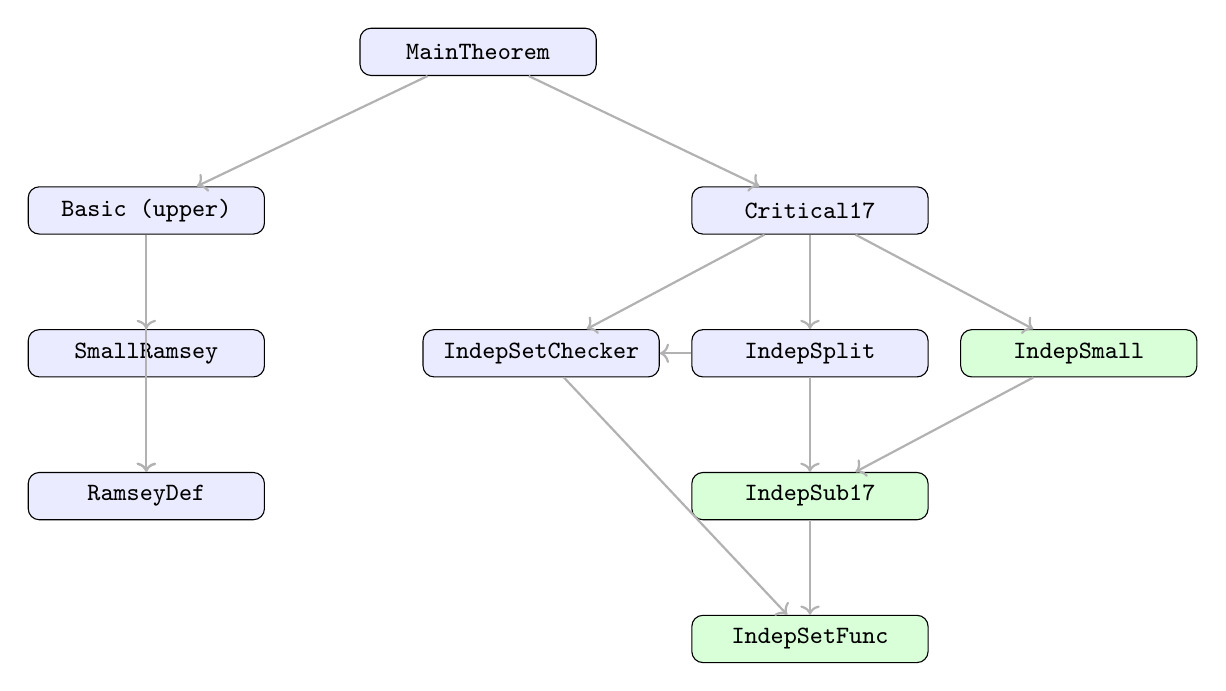
\begin{tikzpicture}[
  node distance=1.4cm and 1.8cm,
  box/.style={draw, rounded corners, fill=blue!8, minimum width=3.0cm,
              minimum height=0.6cm, font=\small\ttfamily, align=center},
  nomath/.style={draw, rounded corners, fill=green!15, minimum width=3.0cm,
                 minimum height=0.6cm, font=\small\ttfamily, align=center},
  arr/.style={->, thick, gray!60},
]
\node[box]    (main)    {MainTheorem};
\node[box,    below left=1.4cm and 1.2cm of main]  (basic)   {Basic (upper)};
\node[box,    below right=1.4cm and 1.2cm of main] (c17)     {Critical17};
\node[box,    below=1.2cm of basic]      (small)   {SmallRamsey};
\node[box,    below left=1.2cm and 0.4cm of c17]   (checker) {IndepSetChecker};
\node[box,    below=1.2cm of c17]        (split)   {IndepSplit};
\node[nomath, below right=1.2cm and 0.4cm of c17]  (indsmall){IndepSmall};
\node[nomath, below=1.2cm of split]      (sub17)   {IndepSub17};
\node[nomath, below=1.2cm of sub17]      (func)    {IndepSetFunc};
\node[box,    below=1.2cm of small]      (rdef)    {RamseyDef};

\draw[arr] (main)    -- (basic);
\draw[arr] (main)    -- (c17);
\draw[arr] (basic)   -- (small);
\draw[arr] (basic)   -- (rdef);
\draw[arr] (c17)     -- (checker);
\draw[arr] (c17)     -- (split);
\draw[arr] (c17)     -- (indsmall);
\draw[arr] (split)   -- (checker);
\draw[arr] (split)   -- (sub17);
\draw[arr] (checker) -- (func);
\draw[arr] (sub17)   -- (func);
\draw[arr] (indsmall)-- (sub17);
\draw[arr] (small)   -- (rdef);
\end{tikzpicture}
\caption{Module dependency graph.
  Green nodes (no Mathlib imports) run kernel evaluation with low memory.
  The blue nodes import Mathlib but are not directly involved in
  kernel-evaluated computations.}
\label{fig:modules}
\end{figure}

\subsection{Reviewer Reproducibility Checklist}
\label{sec:repro}

For ATP/ITP audit, the following checks are sufficient to validate this paper's
central trust claims:

\begin{lstlisting}
lake build
lake env lean Ramsey36/MainTheorem.lean
-- Expected in output:
-- 'ramsey_three_six' depends on axioms:
--   [propext, Classical.choice, Quot.sound]

rg -n "native_decide|Lean.ofReduceBool|sorry|admit" \
  Ramsey36 Ramsey36.lean Main.lean -g "*.lean"
-- Expected: no matches
\end{lstlisting}

% ================================================================
\section{The Lower Bound: The Graver--Yackel Graph}
\label{sec:lower}

The lower bound $R(3,6) \geq 18$ is witnessed by the \emph{Graver--Yackel graph}:
a 17-vertex, 5-regular, triangle-free graph with independence number~5,
constructed in~\cite{graver1968}.

\subsection{Definition in Lean}

We define the graph via an explicit neighborhood table:

\begin{lstlisting}
-- Critical17.lean
def neighbors17 (v : Fin 17) : Finset (Fin 17) :=
  if v = 0 then {9, 14, 15, 16}
  else if v = 1 then {7, 11, 13, 16}
  else if v = 2 then {8, 10, 12, 15}
  -- ...
  else {0, 1, 3, 4, 10}   -- v = 16

def adj17 (v w : Fin 17) : Prop := w in neighbors17 v

def criticalGraph17 : SimpleGraph (Fin 17) where
  Adj    := adj17
  symm   := by intro v w h; exact (neighbors17_symm v w).mp h
  loopless := by
    constructor; intro v h
    unfold adj17 neighbors17 at h
    fin_cases v <;> simp at h
\end{lstlisting}

\noindent
Symmetry of \lean{neighbors17} is proved by
\lean{fin\_cases v <;> fin\_cases w <;> decide},
enumerating all $17 \times 17 = 289$ pairs.
Each goal is a decidable finset-membership check and runs quickly.

\subsection{The Lower Bound Argument}

With the two key properties established (\Cref{sec:checker}), the lower bound
follows by a subgraph embedding argument: if $n \leq 17$, then the
Graver--Yackel graph maps into $K_n$ via \lean{Fin.castLE}, and the Ramsey
property pulls back through \lean{SimpleGraph.comap}.

\begin{lstlisting}
lemma not_hasRamseyProperty_17 :
    not HasRamseyProperty 3 6 criticalGraph17 := by
  unfold HasRamseyProperty; push_neg
  constructor
  . intro s h; exact criticalGraph17_triangleFree s h
  . intro s h; exact criticalGraph17_no_6_indep s h
\end{lstlisting}

% ================================================================
\section{The IndepSetChecker Architecture}
\label{sec:checker}

The two key properties of the Graver--Yackel graph---triangle-freeness and
absence of a 6-independent set---are combinatorial facts about a 17-vertex graph.
This section describes our approach to verifying them in Lean's trusted kernel,
without extra axioms.

\subsection{The Problem with Naive Decidability}
\label{sec:checker:problem}

Both \lean{TriangleFree} and \lean{NoKIndepSet 6} are decidable via
Mathlib's \lean{Fintype} machinery.
In principle, \lean{by decide} should suffice.
In practice it does not:

\begin{itemize}
\item \textbf{Subset enumeration.}
  Mathlib's \lean{IndepSetFree} instance checks all subsets of size $k$.
  For $n = 17$, $k = 6$: $\binom{17}{6} = 12{,}376$ subsets.
  The kernel exhausts memory before completing the check.

\item \textbf{\lean{native\_decide}.}
  Lean's \lean{native\_decide} compiles the check to native code and runs it
  outside the kernel.
  It succeeds, but introduces the axiom \lean{Lean.ofReduceBool}:
  this enlarges the trusted computing base beyond kernel reduction.
  In this artifact we avoid that path and keep theorem checking kernel-native.
\end{itemize}

\subsection{Four-File Architecture}
\label{sec:checker:arch}

Our solution is a custom backtracking search with a kernel-verifiable
correctness proof.
The design separates \emph{computation} (no Mathlib) from
\emph{correctness} (with Mathlib):

\begin{center}
\begin{tabular}{lrl}
\toprule
File & Lines & Role \\
\midrule
\texttt{IndepSetFunc.lean}    & 38  & Search function; \emph{no} Mathlib \\
\texttt{IndepSub17.lean}      & 88  & 12 sub-problems via \lean{decide}; no Mathlib \\
\texttt{IndepSmall.lean}      & 93  & Small Ramsey checks; no Mathlib \\
\texttt{IndepSplit.lean}      & 32  & Combines sub-problems; imports Mathlib \\
\texttt{IndepSetChecker.lean} & 222 & Correctness and bridge; imports Mathlib \\
\bottomrule
\end{tabular}
\end{center}

\medskip\noindent
\textbf{The critical design constraint:}
files that execute \lean{by decide} computations (\texttt{IndepSub17.lean},
\texttt{IndepSmall.lean}) import \emph{only} \texttt{IndepSetFunc.lean}.
Mathlib's compiled \texttt{.olean} files occupy approximately 5\,GB of virtual memory.
Without them, the kernel evaluates Boolean computations in only $\sim\!100$\,MB,
staying well within limits.

\subsection{The Search Function}
\label{sec:checker:func}

The heart of the approach is \lean{hasIndepSetAux} in \texttt{IndepSetFunc.lean},
given here in full:

\begin{lstlisting}
-- IndepSetFunc.lean (complete listing)

/-- Backtracking search: returns `true` iff an independent set of size
    `remaining` exists among vertices {start, ..., n-1} extending `chosen`.
    Recursion depth: O(n), not O(2^n). -/
def hasIndepSetAux (n : Nat) (adj : Fin n -> Fin n -> Bool)
    (remaining : Nat) (start : Nat) (chosen : List (Fin n)) : Nat -> Bool
  | 0        => if remaining = 0 then true else false
  | fuel + 1 =>
    if remaining = 0 then true
    else if h : start < n then
      if n - start < remaining then false        -- pigeonhole prune
      else
        let v : Fin n := <<start, h>>
        let compatible := chosen.all (fun w => !adj v w)
        if compatible then
          hasIndepSetAux n adj (remaining - 1) (start + 1) (v :: chosen) fuel ||
          hasIndepSetAux n adj remaining       (start + 1) chosen         fuel
        else
          hasIndepSetAux n adj remaining       (start + 1) chosen         fuel
    else false

def hasIndepSet (n : Nat) (adj : Fin n -> Fin n -> Bool) (k : Nat) : Bool :=
  hasIndepSetAux n adj k 0 [] (n + 1)
\end{lstlisting}

\noindent
We explain the key design choices:

\paragraph{Parameters.}
\begin{itemize}
  \item \lean{remaining}: how many more vertices still need to be selected.
  \item \lean{start}: the current candidate vertex index (we only look
        at vertices $\geq \lean{start}$, enumerating each subset exactly
        once in lexicographic order).
  \item \lean{chosen}: the list of already-selected vertices.
  \item \lean{fuel}: a syntactic termination counter initialized to $n+1$.
        This keeps recursion depth $O(n)$.
\end{itemize}

\paragraph{Pigeonhole pruning.}
The check \lean{if n - start < remaining then false} terminates branches
where fewer vertices remain than we still need.
This embeds the pigeonhole principle directly into the search: if only $m$
candidate vertices remain ($m < \lean{remaining}$), no independent set of
the required size can exist.

\paragraph{Boolean adjacency.}
The search takes \lean{adj : Fin n -> Fin n -> Bool} rather than
\lean{G.Adj : V -> V -> Prop}.
Boolean functions reduce in the kernel with $O(1)$ cost per lookup
(a single pattern match), whereas propositional adjacency via
\lean{Finset.mem} requires traversing a linked list.
We bridge back to \lean{SimpleGraph} after the computation
(\Cref{sec:checker:bridge}).

\paragraph{Fuel-based recursion.}
Lean requires structural termination arguments.
Using a \lean{Nat} fuel counter decremented at each vertex step
makes the function structurally recursive.
Since \lean{start} advances by~1 per step and $\lean{start} \leq n$,
fuel $n+1$ always suffices.

\subsection{Sub-Problem Splitting}
\label{sec:checker:split}

Even with the Mathlib-free design, a single \lean{decide} on
\lean{hasIndepSet 17 adj17Bool 6} causes kernel out-of-memory.
The search tree has too many nodes for a monolithic evaluation.

The solution: condition on the \emph{first selected vertex} (vertices~$0$
through~$11$), splitting the search into 12 sub-problems.
Vertices $\geq 12$ cannot start a 6-independent set by pigeonhole:
only $17 - 12 = 5 < 6$ vertices remain.

Each sub-problem fixes vertex~$i$ as selected and asks whether 5 more
independent vertices exist among $\{i+1,\ldots,16\}$:

\begin{lstlisting}
-- IndepSub17.lean

/-- Direct Bool adjacency for the Graver-Yackel 17-vertex graph. -/
def adj17Bool (v w : Fin 17) : Bool :=
  match v.val, w.val with
  | 0, 9  | 0, 14 | 0, 15 | 0, 16 => true
  | 1, 7  | 1, 11 | 1, 13 | 1, 16 => true
  -- ... (all 43 edges, both directions)
  | _, _ => false

set_option maxHeartbeats 800000 in
theorem sub17_0 :
    hasIndepSetAux 17 adj17Bool 5 1 [<<0, by omega>>] 17 = false := by decide

set_option maxHeartbeats 800000 in
theorem sub17_1 :
    hasIndepSetAux 17 adj17Bool 5 2 [<<1, by omega>>] 16 = false := by decide

-- ... sub17_2 through sub17_10 ...

set_option maxHeartbeats 200000 in
theorem sub17_11 :
    hasIndepSetAux 17 adj17Bool 5 12 [<<11, by omega>>] 6 = false := by decide
\end{lstlisting}

\noindent
Each sub-problem has at most $\sim\!970$ search nodes and verifies in under
one second.
Heartbeat limits decrease for later vertices (reflecting the shrinking
search space).

Defining adjacency as an exhaustive \lean{match} rather than via
\lean{Finset.mem} avoids linked-list traversal overhead during kernel
evaluation.

\subsection{Structural Decomposition: Combining Sub-Problems}
\label{sec:checker:decomp}

The 12 sub-problems are combined in \texttt{IndepSplit.lean} using the
structural decomposition lemma from \texttt{IndepSetChecker.lean}:

\begin{lstlisting}
-- IndepSetChecker.lean

/-- If both the include-v and skip-v branches return false, the full
    call returns false.  Used to chain sub-problem results. -/
theorem hasIndepSetAux_false_of_compat
    {n : Nat} {adj : Fin n -> Fin n -> Bool}
    {remaining start fuel : Nat} {chosen : List (Fin n)}
    (h_rem    : remaining /= 0)
    (h_start  : start < n)
    (h_pig    : not (n - start < remaining))
    (h_compat : (chosen.all fun w => !adj <<start, h_start>> w) = true)
    (h_inc  : hasIndepSetAux n adj (remaining-1) (start+1)
                (<<start, h_start>> :: chosen) fuel = false)
    (h_skip : hasIndepSetAux n adj remaining (start+1) chosen fuel = false) :
    hasIndepSetAux n adj remaining start chosen (fuel + 1) = false
\end{lstlisting}

\noindent
The combination proof chains 12 applications of this lemma:

\begin{lstlisting}
-- IndepSplit.lean

theorem hasIndepSet_17_adj17Bool_6_false :
    hasIndepSet 17 adj17Bool 6 = false := by
  show hasIndepSetAux 17 adj17Bool 6 0 [] 18 = false
  exact hasIndepSetAux_false_of_compat (...) sub17_0 <|
  hasIndepSetAux_false_of_compat (...) sub17_1 <|
  -- ...
  hasIndepSetAux_false_of_compat (...) sub17_11 <|
  hasIndepSetAux_false_of_pig (by decide) (by omega) (by omega)
\end{lstlisting}

\noindent
The final \lean{hasIndepSetAux\_false\_of\_pig} handles the pigeonhole base
case: no 6-IS can start with a vertex $\geq 12$.

\subsection{Correctness: The Completeness Theorem}
\label{sec:checker:correct}

The search function is \emph{sound} by construction (when it returns
\lean{true}, \lean{chosen} is a valid independent set by invariant of the
loop---each vertex is added only when compatible with all prior choices).
This direction is \emph{not} stated as a separate theorem because all
applications in this work only use \lean{false} results.
The non-trivial and mechanically verified direction is \emph{completeness}:
if a $k$-independent set exists, the search returns \lean{true}.
This is the theorem that makes the entire architecture formally sound:
a \lean{false} result is not merely trusted by fast execution---it is an
axiom-free kernel theorem whose proof term Lean's type-checker certifies.
Without this theorem, the checker would be an unverified oracle.

\begin{lstlisting}
-- IndepSetChecker.lean

/-- If a k-independent set exists, the backtracking search returns true. -/
theorem hasIndepSetAux_complete
    {n : Nat} {adj : Fin n -> Fin n -> Bool}
    {remaining start fuel : Nat} {chosen : List (Fin n)}
    {s : Finset (Fin n)}
    (h_fuel   : n <= start + fuel)
    (h_card   : s.card = remaining)
    (h_ge     : forall v in s, start <= v.val)
    (h_indep  : forall v in s, forall w in s,
                  v /= w -> adj v w = false)
    (h_compat : forall v in s, forall w in chosen,
                  adj v w = false) :
    hasIndepSetAux n adj remaining start chosen fuel = true
\end{lstlisting}

\begin{proof}[Proof sketch]
By induction on \lean{fuel}.
\textbf{Base case} (\lean{fuel = 0}): if any vertex of $s$ remained,
it would need index $\geq \lean{start} \geq n$ (by \lean{h\_fuel}),
contradicting the type bound on \lean{Fin n}.
Hence $s$ is empty, so \lean{remaining = 0}, and the function returns
\lean{true}.

\textbf{Inductive step}: the pigeonhole guard passes since $|s| =
\lean{remaining}$ elements all have index $\geq \lean{start}$.
Case-split on whether $\lean{start} \in s$:
\begin{itemize}
  \item If yes: \lean{h\_compat} ensures the compatibility check passes.
    Apply the inductive hypothesis to $s \setminus \{\lean{start}\}$ to
    obtain \lean{true} for the include branch.
  \item If no: all elements of $s$ have index $\geq \lean{start} + 1$.
    Apply the inductive hypothesis to $s$ for the skip branch.
\end{itemize}
\end{proof}

\noindent
The contrapositive is what we need: if \lean{hasIndepSetAux~...~= false},
then no $k$-independent set of the required form exists.

\subsection{Bridge to Mathlib's \texttt{SimpleGraph}}
\label{sec:checker:bridge}

The final step connects the Boolean computation to Mathlib's propositional
\lean{NoKIndepSet} predicate.
We generalize the bridge to accept any Boolean adjacency function that agrees
pointwise with the graph's adjacency relation:

\begin{lstlisting}
-- IndepSetChecker.lean

/-- If `adj` agrees with `decide (G.Adj . .)` pointwise,
    and the checker returns false, then G has no k-independent set. -/
theorem noKIndepSet_of_adj_checker_false
    {n k : Nat} {G : SimpleGraph (Fin n)} [DecidableRel G.Adj]
    {adj : Fin n -> Fin n -> Bool}
    (hadj : forall v w : Fin n, adj v w = decide (G.Adj v w))
    (h    : hasIndepSet n adj k = false) :
    NoKIndepSet k G := by
  apply noKIndepSet_of_checker_false
  have heq : adj = fun v w => decide (G.Adj v w) :=
    funext (fun v => funext (fun w => hadj v w))
  rwa [<- heq]
\end{lstlisting}

\noindent
In \texttt{Critical17.lean}, we instantiate this with a \lean{decide}
proof covering all $17 \times 17 = 289$ pairs:

\begin{lstlisting}
-- Critical17.lean

/-- adj17Bool agrees with criticalGraph17.Adj on all 289 pairs.
    Each pair costs O(5) kernel steps (degree-5 finset lookup). -/
private lemma adj17Bool_spec :
    forall v w : Fin 17,
      adj17Bool v w = decide (criticalGraph17.Adj v w) := by decide

lemma criticalGraph17_no_6_indep : NoKIndepSet 6 criticalGraph17 :=
  noKIndepSet_of_adj_checker_false adj17Bool_spec
    hasIndepSet_17_adj17Bool_6_false
\end{lstlisting}

\noindent
The \lean{decide} call in \lean{adj17Bool\_spec} performs
$17 \times 17 = 289$ finset membership lookups, each of cost $O(5)$
(the graph is 5-regular), for $\sim\!1{,}500$ total kernel steps---well
within limits.

\begin{remark}[A crucial pitfall with \lean{decide} and free variables]
\label{rem:freevar}
Lean's \lean{decide} tactic requires a \emph{closed} proposition (no free variables).
Writing

\begin{lstlisting}
-- WRONG: v and w are free variables in the local context
private lemma adj17Bool_spec (v w : Fin 17) :
    adj17Bool v w = decide (criticalGraph17.Adj v w) := by decide
\end{lstlisting}

\noindent
fails with \texttt{Expected type must not contain free variables}.
The fix is to lift the universal quantifier into the proposition itself:

\begin{lstlisting}
-- CORRECT: closed proposition, decide works
private lemma adj17Bool_spec :
    forall v w : Fin 17,
      adj17Bool v w = decide (criticalGraph17.Adj v w) := by decide
\end{lstlisting}
\end{remark}

\subsection{Triangle-Freeness via the Complement}
\label{sec:checker:tf}

A triangle in $G$ is a 3-clique, which corresponds to a 3-independent-set
in the \emph{complement} graph.
We exploit this duality to reuse the same checker infrastructure:

\begin{lstlisting}
-- IndepSmall.lean

/-- Complement adjacency: edge iff NOT adjacent in the original graph.
    A 3-IS in adj17NotBool = a 3-clique in adj17Bool = a triangle. -/
def adj17NotBool (v w : Fin 17) : Bool := !adj17Bool v w

-- Single fast check: the complement has 93 edges, 3-clique absent.
set_option maxHeartbeats 400000 in
theorem hasIndepSet_17_adj17NotBool_3_false :
    hasIndepSet 17 adj17NotBool 3 = false := by decide
\end{lstlisting}

\noindent
The corresponding bridge theorem and instantiation:

\begin{lstlisting}
-- IndepSetChecker.lean

theorem triangleFree_of_adj_checker_false
    {n : Nat} {G : SimpleGraph (Fin n)} [DecidableRel G.Adj]
    {adjNot : Fin n -> Fin n -> Bool}
    (hadj : forall v w : Fin n, adjNot v w = !decide (G.Adj v w))
    (h : hasIndepSet n adjNot 3 = false) : TriangleFree G

-- Critical17.lean

private lemma adj17NotBool_spec :
    forall v w : Fin 17,
      adj17NotBool v w = !decide (criticalGraph17.Adj v w) := by decide

lemma criticalGraph17_triangleFree : TriangleFree criticalGraph17 :=
  triangleFree_of_adj_checker_false adj17NotBool_spec
    hasIndepSet_17_adj17NotBool_3_false
\end{lstlisting}

\subsection{Summary of the Architecture}

The IndepSetChecker achieves kernel-verified combinatorial decidability
through four interlocking principles:

\begin{enumerate}
\item \textbf{Separation of computation and verification.}
  The search function (no Mathlib, $\sim\!100$\,MB) and correctness proof
  (with Mathlib) live in separate files.

\item \textbf{Fuel-bounded backtracking.}
  Linear recursion depth avoids the $O(2^n)$ stack blow-up of naive
  enumeration.

\item \textbf{Structural decomposition.}
  Large searches are split into small sub-problems, each independently
  verifiable by \lean{decide}, then combined via a chain of bridge lemmas.

\item \textbf{Complement duality.}
  Triangle-freeness reuses the independent-set checker on the complement,
  requiring no separate infrastructure.
\end{enumerate}

% ================================================================
\section{The Upper Bound: Formalizing Cariolaro's Proof}
\label{sec:upper}

The upper bound $R(3,6) \leq 18$ is the bulk of the formalization,
occupying \texttt{Basic.lean} ($\sim\!12{,}900$ lines).
We outline the three main claims from Cariolaro's proof~\cite{cariolaro1999}
and note key Lean-specific aspects.

\subsection{Setup}

Throughout, $G$ is a triangle-free graph on 18 vertices with no
6-independent set.
We derive a contradiction.

A foundational observation from \texttt{RamseyDef.lean}:

\begin{lstlisting}
/-- In a triangle-free graph, the neighborhood of any vertex is independent. -/
lemma neighborSet_indep_of_triangleFree
    {G : SimpleGraph V} (h : TriangleFree G) (v : V) :
    G.IsIndepSet (G.neighborSet v)
\end{lstlisting}

\noindent
Since $N(v)$ is independent and $G$ has no 6-IS, we immediately get
$\deg(v) \leq 5$ for all $v$.

\subsection{Claim 1: \texorpdfstring{$G$ is 5-Regular}{G is 5-Regular}}

\begin{lemma}[Formalized as \lean{claim1\_five\_regular}]
$G$ is 5-regular.
\end{lemma}

\textbf{Upper bound on degree.}
$N(v)$ is independent with $|N(v)| = \deg(v)$, so $\deg(v) \leq 5$.

\textbf{Lower bound on degree.}
Suppose $\deg(v) < 5$.
Let $H = G - N[v]$; then $|H| \geq 13$.
\begin{itemize}
  \item If $|H| \geq 14 = \RR{3}{5}$: since $\RR{3}{5} = 14$ is formalized
    (\Cref{sec:small}), $H$ contains a 5-IS, which together with $v$ gives
    a 6-IS---contradiction.
  \item If $|H| = 13$ (so $\deg(v) = 4$): $H$ must be the unique
    $\RR{3}{5}$-critical graph (Paley(13), 4-regular).
    A counting argument via a neighbor $t \in N(v)$ constructs a 6-IS
    from $(N(v) \setminus \{t\}) \cup \{t_1, t_2, t_3\}$ where $t_i \in H$
    are neighbors of $t$.
\end{itemize}

\noindent
This argument relies directly on the previously formalized $\RR{3}{5} = 14$,
illustrating how the small Ramsey results feed into the main proof.

\subsection{Claim 2: Neighbor Structure}

\begin{lemma}[Formalized as \lean{claim2\_neighbor\_structure}]
For any non-adjacent pair $u, v$: $1 \leq |N(u) \cap N(v)| \leq 2$.
Moreover, for any vertex $v$, exactly 4 non-neighbors share exactly 1 common
neighbor with $v$ (the set $P$), and 8 non-neighbors share exactly 2 (the
set $Q \cup W$).
\end{lemma}

\begin{itemize}
\item \textbf{Lower bound.} If $N(u) \cap N(v) = \emptyset$, then
  $\{u\} \cup N(u)$ is a 6-IS.
\item \textbf{Upper bound.} If $|N(u) \cap N(v)| \geq 3$, then
  $G - N[u,v]$ has $\geq 9 = \RR{3}{4}$ vertices, containing a 4-IS;
  together with $u,v$ this gives a 6-IS.
\end{itemize}

\noindent
The counting uses \lean{commonNeighbors} from \texttt{RamseyDef.lean}
and a double-counting argument on edges between $G - N[v]$ and $N[v]$.

\subsection{Claim 3: \texorpdfstring{$P$ Induces a 4-Cycle}{P Induces a 4-Cycle}}

\begin{lemma}[Formalized as \lean{claim3\_four\_cycle}]
The set $P$ of 4 non-neighbors of $v$ that each share exactly one common
neighbor with $v$ induces a 4-cycle in $G$.
\end{lemma}

The key tool is the \textbf{FiveCycleLemma} (\texttt{FiveCycleLemma.lean}):

\begin{theorem}[Five-cycle structure]
In a 5-vertex triangle-free graph with no 3-independent set, every vertex
has degree exactly~2 (i.e., the graph is the 5-cycle $C_5$).
\end{theorem}

\begin{proof}[Proof sketch]
\textit{Min degree $\geq 2$.} If $\deg(v) \leq 1$, the 3 non-neighbors of $v$
contain at most 1 edge (triangle-free), leaving a 3-IS with $v$.
\textit{Max degree $\leq 2$.} If $\deg(v) \geq 3$, three neighbors form
a 3-IS since $N(v)$ is independent (triangle-free).
\end{proof}

\noindent
The lemma is applied to the 5-vertex induced subgraph on $\{v\} \cup P$:
each $p_i \in P$ has exactly one neighbor in $N(v)$ (by definition of $P$),
so the $p_i$'s have degree 2 in this subgraph---forcing the 4-cycle structure.

\subsection{Final Contradiction}

Cariolaro's labeling:
$V(G) = \{v, t, s_1, s_2, s_3, s_4, t_1, t_2, t_3, t_4,
           p_1, p_2, p_3, p_4, w_1, w_2, w_3, w_4\}$

\noindent
where $N(v) = \{t, s_1, s_2, s_3, s_4\}$, $N(t) \setminus \{v\}
= \{t_1, t_2, t_3, t_4\}$, $P = \{p_1, p_2, p_3, p_4\}$ induces the
4-cycle $p_1 p_2 p_3 p_4 p_1$, and $W = \{w_1, w_2, w_3, w_4\}$.

A careful case analysis (formalized as \lean{final\_contradiction} in
\texttt{Basic.lean}) shows:
$w_1$ is adjacent to $s_3$ and $t_1$, and the edge $w_1 s_2 \in E(G)$
forces $s_2 t_1 \in E(G)$.
But then $s_2$ and $p_1$ share three common neighbors $\{p_2, w_1, t_1\}$,
contradicting Claim~2. \qed

\noindent
The main upper bound theorem is then:

\begin{lstlisting}
theorem hasRamseyProperty_3_6_18 :
    0 < 18 and forall (G : SimpleGraph (Fin 18)) [DecidableRel G.Adj],
      HasRamseyProperty 3 6 G := by
  constructor
  . simp
  . intro G inst
    by_contra h_not_ramsey
    unfold HasRamseyProperty at h_not_ramsey; push_neg at h_not_ramsey
    rcases h_not_ramsey with <<h_no_clique, h_no_indep>>
    have h_tri : TriangleFree G     := fun t ht => h_no_clique t ht
    have h_no6 : NoKIndepSet 6 G    := fun t ht => h_no_indep  t ht
    have h_reg : IsKRegular G 5     := claim1_five_regular h_tri h_no6
    exact final_contradiction h_reg h_tri h_no6
\end{lstlisting}

% ================================================================
\section{Small Ramsey Numbers as Dependencies}
\label{sec:small}

The upper bound for $R(3,6) = 18$ (specifically, Claim~1) relies on the
values of $\RR{3}{3} = 6$, $\RR{3}{4} = 9$, and $\RR{3}{5} = 14$.
All three are fully formalized in \texttt{SmallRamsey.lean} using the same
IndepSetChecker architecture, with computations in \texttt{IndepSmall.lean}.

\begin{center}
\begin{tabular}{llll}
\toprule
Theorem & Critical graph & $n$ & Computation \\
\midrule
$\RR{3}{3} = 6$ & $C_5$ (5-cycle)    &  5 & \lean{hasIndepSet 5 adj5Bool 3 = false} \\
$\RR{3}{4} = 9$ & $C_8(1,4)$         &  8 & \lean{hasIndepSet 8 adj8Bool 4 = false} \\
$\RR{3}{5} = 14$ & Paley(13)         & 13 & \lean{hasIndepSet 13 adj13Bool 5 = false} \\
\bottomrule
\end{tabular}
\end{center}

\noindent
For example, the Paley(13) computation (quadratic-residue adjacency mod 13):

\begin{lstlisting}
-- IndepSmall.lean

def adj13Bool (v w : Fin 13) : Bool :=
  match v.val, w.val with
  | 0, 1  | 0, 5  | 0, 8  | 0, 12 => true
  | 1, 0  | 1, 2  | 1, 6  | 1,  9 => true
  -- ...
  | _, _ => false

set_option maxHeartbeats 400000 in
theorem hasIndepSet_13_adj13Bool_5_false :
    hasIndepSet 13 adj13Bool 5 = false := by decide
\end{lstlisting}

\noindent
The structure---explicit adjacency table, no Mathlib, \lean{by decide}---is
identical to the 17-vertex case, but fits in a single \lean{decide} call
since $\binom{13}{5}$ is small enough.

% ================================================================
\section{Equivalence with the Textbook Definition}
\label{sec:textbook}

A potential objection to the \lean{sInf}-based definition of \lean{ramseyNumber} is
that it might not match the standard combinatorial definition in the literature.
The file \texttt{RamseyAlt.lean} closes this gap formally.

\subsection{The Textbook Definition}

Following Radziszowski's survey~\cite{radziszowski}, $R(k,l)$ is the
\emph{least positive integer $n$} such that every graph on $n$ vertices
contains either a $k$-clique or an $l$-independent set.
Translated directly into Lean:

\begin{lstlisting}
-- RamseyAlt.lean

/-- Classical characterization (Radziszowski 1994):
    R(k,l) is the LEAST positive n such that
    every n-vertex graph has a k-clique or l-IS.
    (i)  n > 0
    (ii) every n-vertex graph has the Ramsey property
    (iii) for each 0 < m < n, some m-vertex graph lacks it -/
def IsRamseyNumber (k l n : Nat) : Prop :=
  0 < n and
  (forall (G : SimpleGraph (Fin n)) [DecidableRel G.Adj],
    HasRamseyProperty k l G) and
  (forall m : Nat, 0 < m -> m < n ->
    exists (G : SimpleGraph (Fin m))
           (_ : DecidableRel G.Adj),
      not HasRamseyProperty k l G)
\end{lstlisting}

\noindent
Condition~(iii) is the critical one: it certifies that $n$ is truly minimal.

\subsection{Instance Independence}

\lean{HasRamseyProperty k l G} is defined as
$(\exists s,\, G.\text{IsNClique}\; k\; s) \lor (\exists s,\, G.\text{IsNIndepSet}\; l\; s)$,
which does not reference the \lean{DecidableRel G.Adj} instance.
Therefore the proposition is instance-independent:

\begin{lstlisting}
lemma hasRamseyProperty_instIndep {V : Type*}
    (k l : Nat) (G : SimpleGraph V)
    (inst1 inst2 : DecidableRel G.Adj) :
    @HasRamseyProperty V k l G inst1 <->
    @HasRamseyProperty V k l G inst2 := Iff.rfl
\end{lstlisting}

\noindent
This means the set over which \lean{sInf} is taken in
\lean{ramseyNumber} is unaffected by instance choices.

\subsection{Equivalence Theorem}

\begin{theorem}[Formalized as \lean{isRamseyNumber\_iff\_eq\_ramseyNumber}]
When the Ramsey set is nonempty,
$\lean{IsRamseyNumber}\; k\; l\; n \iff n = \lean{ramseyNumber}\; k\; l$.
\end{theorem}

\begin{proof}[Proof sketch]
\emph{Forward.}
If $n$ satisfies conditions (i)--(iii), then $n$ belongs to the Ramsey set,
so $\lean{sInf} \leq n$.
If $\lean{ramseyNumber} < n$, condition~(iii) produces a graph on
$\lean{ramseyNumber}$ vertices lacking the Ramsey property,
contradicting that $\lean{ramseyNumber}$ is \emph{in} the Ramsey set (condition~(ii)).
Hence $n = \lean{ramseyNumber}$.

\emph{Backward.}
$\lean{sInf}$ of a nonempty subset of $\mathbb{N}$ belongs to the set
(\lean{Nat.sInf\_mem}) and is a lower bound (\lean{Nat.sInf\_le}).
These immediately give conditions~(i)--(iii).
\end{proof}

\subsection{Main Instantiation}

\begin{lstlisting}
-- RamseyAlt.lean

theorem isRamseyNumber_3_6_18 : IsRamseyNumber 3 6 18 :=
  (isRamseyNumber_iff_eq_ramseyNumber
      ramseySet_3_6_nonempty').mpr
    ramsey_three_six.symm
\end{lstlisting}

\noindent
Verified axiom footprint:

\begin{lstlisting}
#print axioms isRamseyNumber_3_6_18
-- 'isRamseyNumber_3_6_18' depends on axioms:
--   [propext, Classical.choice, Quot.sound]
\end{lstlisting}

\noindent
This confirms that \lean{ramseyNumber 3 6} in our formalization is exactly the
classical combinatorial object defined in the literature.

% ================================================================
\section{Axiom Footprint and Trust}
\label{sec:axioms}

\begin{lstlisting}
#print axioms ramsey_three_six
-- 'ramsey_three_six' depends on axioms:
--   [propext, Classical.choice, Quot.sound]
\end{lstlisting}

\noindent
The three axioms are the standard Lean~4 foundations:
\begin{itemize}
  \item \textbf{\lean{propext}}: logically equivalent propositions are equal.
  \item \textbf{\lean{Classical.choice}}: non-constructive choice, needed
    for \lean{sInf} in the definition of \lean{ramseyNumber}.
  \item \textbf{\lean{Quot.sound}}: quotient soundness, used throughout
    Mathlib's algebra and graph theory infrastructure.
\end{itemize}

\noindent
Notably absent:

\begin{itemize}
  \item \textbf{\lean{Lean.ofReduceBool}}: the axiom introduced by
    \lean{native\_decide}.
    Our use of \lean{by decide} with Mathlib-free sub-problem files
    means all computations are verified by Lean's trusted kernel.
  \item \textbf{\lean{sorry} / custom axioms}: none.
\end{itemize}

\paragraph{Trust discussion.}
Lean's kernel is a small, independently auditable piece of code (the
\emph{trusted computing base}).
A proof accepted by the kernel with the above three axioms carries the same
epistemic status as a traditional mathematical proof in ZFC with
propositional extensionality.
By contrast, \lean{native\_decide} delegates verification to a compiled
binary and therefore depends on additional compiler/runtime trust assumptions.
The IndepSetChecker architecture is specifically designed to avoid this
trust gap.

% ================================================================
\section{Conclusion}
\label{sec:conclusion}

We have presented a complete Lean~4 mechanization of $R(3,6) = 18$,
with axiom footprint confined to the three standard Lean foundations.

The key technical contribution is the \emph{IndepSetChecker}: a reusable,
kernel-efficient framework for combinatorial decidability on graphs,
combining:
\begin{enumerate}
\item a fuel-bounded backtracking search with pigeonhole pruning (Mathlib-free),
\item a completeness theorem (with Mathlib),
\item a structural decomposition principle for splitting large computations, and
\item a clean pointwise bridge from Boolean adjacency to Mathlib's \lean{SimpleGraph}.
\end{enumerate}

\noindent
This architecture addresses a genuine tension in interactive theorem proving:
combinatorial properties of small graphs are in principle decidable,
but naive kernel evaluation is infeasible and \lean{native\_decide} expands
the trusted base.
We thread this needle by separating computation from correctness,
keeping evaluation Mathlib-free, and splitting large computations into
kernel-digestible sub-problems.

\paragraph{Future work.}
The next natural targets are $R(3,7) = 23$ and $R(4,4) = 18$.
The IndepSetChecker scales: $R(3,7)$ would require $\sim\!100$--$200$
sub-problems for the 22-vertex critical graph.
Integration with PBLean~\cite{pblean} via VeriPB certificates is another
avenue, providing an independent computational witness.

% ================================================================
\section*{Acknowledgments}

The authors thank \textbf{Lawrence Paulson} (University of Cambridge) for
the key suggestion to replace \lean{native\_decide} with a verified
backtracking algorithm whose correctness is certified by a completeness theorem
inside the kernel---the design principle at the heart of the IndepSetChecker
architecture.
We thank \textbf{Josef Urban} (Czech Technical University in Prague) for
proposing $R(3,6) = 18$ as a ``proof-of-capacity'' autoformalization
benchmark and for encouraging a machine-verifiable account of the full
formalization pipeline.

\bibliographystyle{plain}
\begin{thebibliography}{10}

\bibitem{cariolaro1999}
D.~Cariolaro.
\newblock On the Ramsey number $R(3,6)$.
\newblock {\em Research Report R-99-2012}, Aalborg University, Denmark, 1999.

\bibitem{greenwood1955}
R.~E. Greenwood and A.~M. Gleason.
\newblock Combinatorial relations and chromatic graphs.
\newblock {\em Canadian Journal of Mathematics}, 7:1--7, 1955.

\bibitem{graver1968}
J.~E. Graver and J.~Yackel.
\newblock Some graph theoretic results associated with Ramsey's theorem.
\newblock {\em Journal of Combinatorial Theory}, 4:125--175, 1968.

\bibitem{radziszowski}
S.~P. Radziszowski.
\newblock Small Ramsey numbers.
\newblock {\em Electronic Journal of Combinatorics}, Dynamic Survey DS1,
  1994 (updated regularly).

\bibitem{lean4}
L.~de~Moura, S.~Ullrich, et~al.
\newblock The {Lean~4} theorem prover and programming language.
\newblock In {\em Proceedings of CADE-28}, 2021.

\bibitem{mathlib}
The Mathlib Community.
\newblock Mathlib: A unified library of mathematics for {Lean~4}.
\newblock \url{https://leanprover-community.github.io/}, 2024.

\bibitem{pblean}
J.~Blanchette, H.~Manthey, S.~Szeider, et~al.
\newblock {PBLean}: Pseudo-Boolean proof checking in {Lean~4}.
\newblock Preprint, 2024--2026.

\end{thebibliography}

\end{document}
